\documentclass[paper=a4, fontsize=11pt]{article} 

\usepackage[T1]{fontenc} 

\usepackage[utf8]{inputenc}
\usepackage[francais]{babel} 
\usepackage{mathtools}
\usepackage{amssymb}
\usepackage{alltt}
\usepackage{float}
\usepackage{graphicx}
\usepackage[colorinlistoftodos]{todonotes}
\usepackage{geometry}
\usepackage{hyperref}
\usepackage{enumitem}

\title{\normalfont \normalsize 
\huge TP 1 - Gradient, Levenberg-Marquardt, Nelder-Mead}

\author{Jules Kozolinsky}

\date{}

\begin{document}
\maketitle

\section{Gradient et règle d'Armijo pour la recherche linéaire approchée}
\subsection{Fonction de Rosenbrock}
\paragraph{Lignes de niveaux de la fonction de Rosenbrock\\}
On remarque sur le graphique ~\ref{étiquette} que les lignes de niveaux ont une forme de crevasse. Il peut donc sembler difficile de trouver le minimum global. 
\begin{figure}[h]
 	\begin{center}
   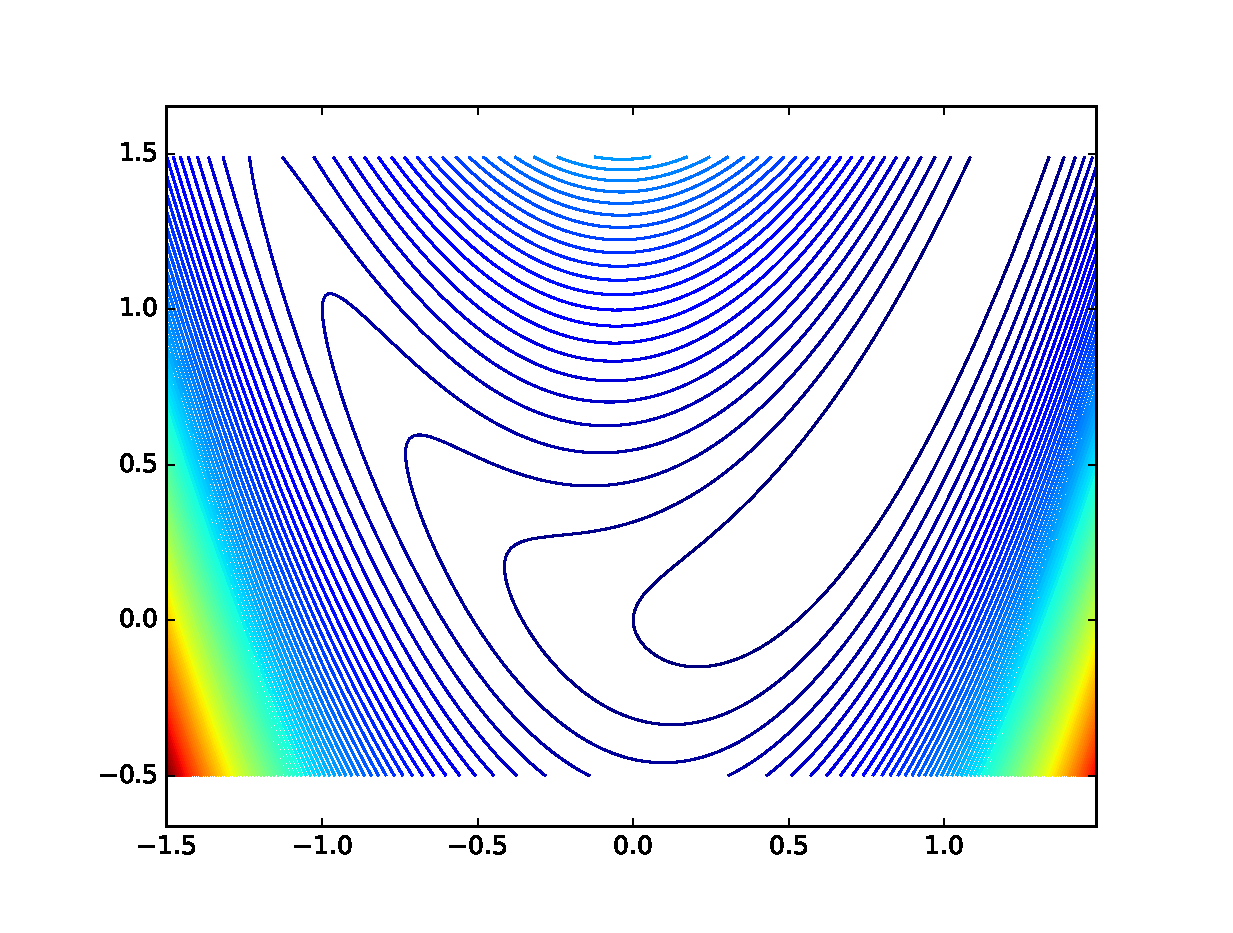
\includegraphics[scale=0.6]{lignes-niveaux-rosenbrock}
   \end{center}
   \caption{\label{étiquette} Lignes de niveaux de la fonction de Rosenbrock}
\end{figure}

\paragraph{Calcul de $\nabla J(\textbf{u})$\\}
On a $J(\textbf{u}) = (1-u_1)^2 + p(u_2 - u_1^2)^2 = 1 - 2u_1 + u_1^2 + pu_2^2 - 2pu_1^2u_2 + pu_1^4$. \\
D'où : 
\begin{itemize}[label=\textbullet]
\item $\frac{\partial J }{\partial u_1} = -2 + 2u_1 - 4pu_1u_2 + 4pu_1^3 = 2(u_1-1) + 4pu_1(u_1^2-u_2) $ 
\item $\frac{\partial J }{\partial u_2} = 2p(u_2-u_1^2)$
\end{itemize}
On remarque que $\nabla J(\textbf{u*}) = \textbf{0}$.

\paragraph{Étude numérique de la suite $(u^k)_k$\\}
On conjecture une convergence de la suite $(u^k)_k$ vers le minimum global $u*$ qui s'effectue très lentement (les itérés $(u^{k})_{k}$ sont en effet très proches). On remarque que les itérés sont orthogonaux aux lignes de niveaux, ce qui s'explique par $u^{k+1}-u^{k} = \rho \frac{\nabla J(u^k)}{\left\|\nabla J(u^k)\right\|}$.\\
\begin{figure}[h]
\begin{center}
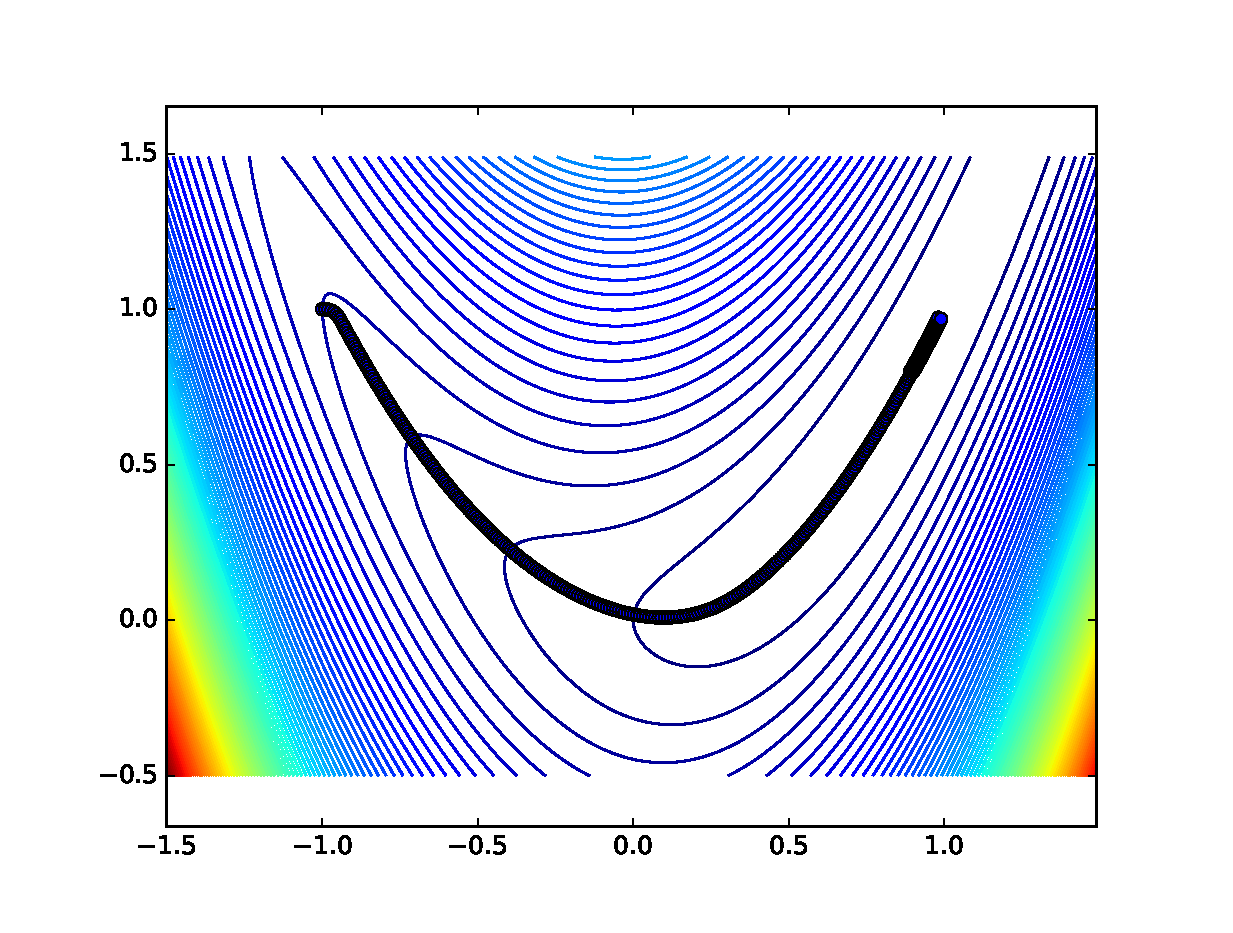
\includegraphics[scale=0.6]{suite-u}
 \end{center}
 \caption{\label{étiquette2} Itérés $(u^{k})_{k\leq500}$ sur les lignes de niveaux de $J$}
\end{figure}

\paragraph{Critère de convergence de la suite $(u^k)_k$\\}
Soit $n$, trouver $k$ tel que $\frac{\left\|\nabla J(u^k)\right\|}{\left\|\nabla J(u^0)\right\|} \leq 10^{-n}$.\\
Pour $ n = 4$, l'algorithme ne termine pas en un temps raisonnable. \\
Pour $ n = 1$, on trouve $k = 229$.

\subsection{Règle d'Armijo}
On observe une fois de plus la converge de la suite $u$ mais cette fois-ci de manière bien plus rapide (surtout lors des premières itérations), ce qui est confirmé par le faible nombre d'itérations nécessaires pour atteindre le critère de convergence avec $n = 4$ (en reprenant les notations précédentes). On trouve $ k = 771$.
\begin{figure}[h]
 	\begin{center}
   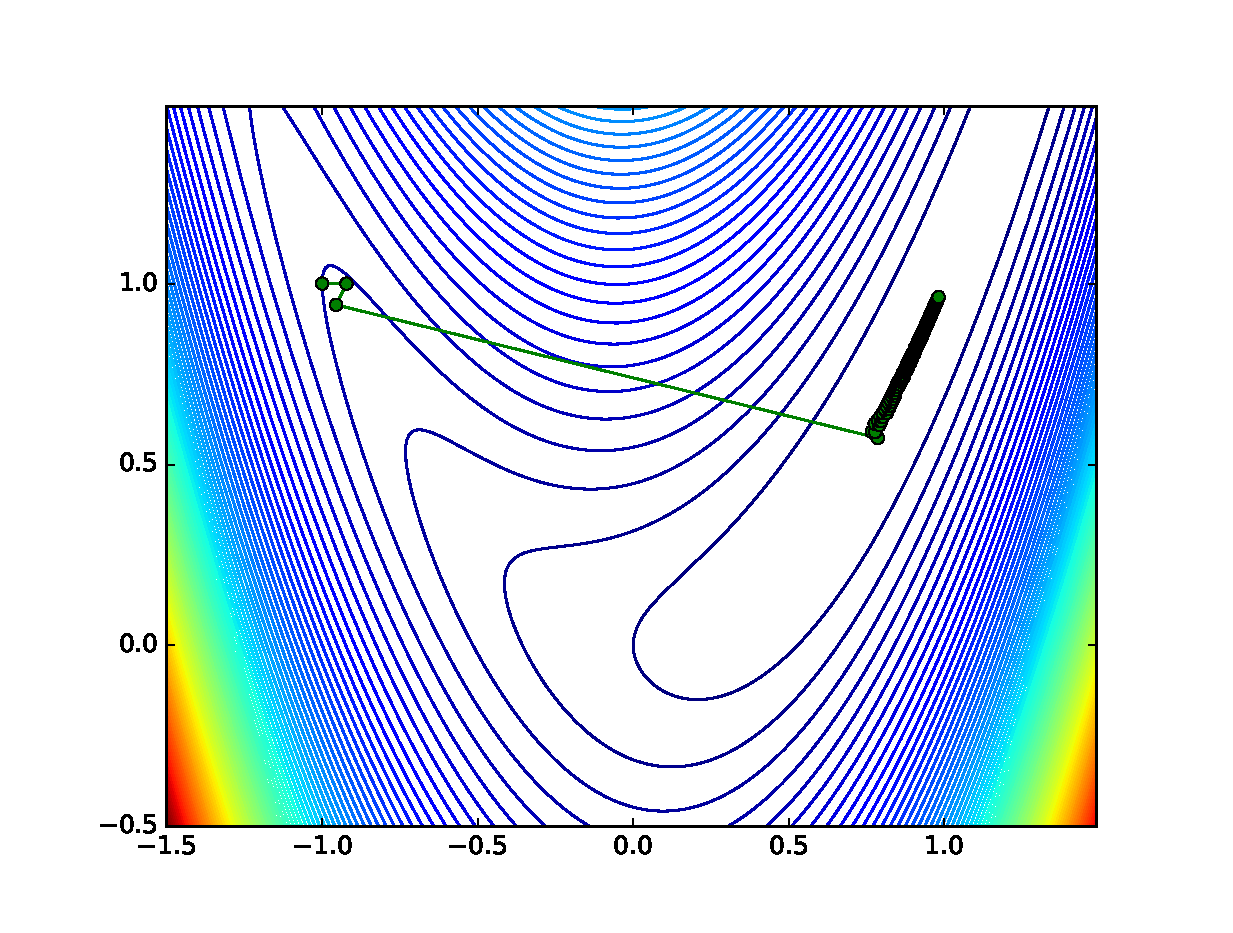
\includegraphics[scale=0.6]{suite-u-armijo}
   \end{center}
   \caption{\label{étiquette} Itérés $(u^{k})_{k\leq500}$ de la règle d'Armijo sur les lignes de niveaux de $J$}
\end{figure}

\section{Régression non linéaire, algorithme de Levenberg-Marquardt}
\paragraph{Calcul de $S^k$\\}
Pour calculer $S^k$, on a besoin de calculer $\nabla\varphi_i(\textbf{u})$ et donc $\frac{\partial f }{\partial\textbf{u}}$.\\
On a : \\
\begin{itemize}[label=\textbullet]
\item $\frac{\partial f }{\partial\alpha_j} = \exp(-\frac{1}{2}\frac{(x-x_j^0)^2}{\sigma_j^2})$ 
\item $\frac{\partial f }{\partial\sigma_j} = \alpha_j\frac{(x-x_j^0)^2}{\sigma_j^3}\exp(-\frac{1}{2}\frac{(x-x_j^0)^2}{\sigma_j^2}) $
\item $\frac{\partial f }{\partial x_j^0} = \alpha_j\frac{x-x_j^0}{\sigma_j^2}\exp(-\frac{1}{2}\frac{(x-x_j^0)^2}{\sigma_j^2})$
\end{itemize}
Pour la règle d'Armijo, on considère la direction de recherche $\textbf{d}^k$ pour atteindre la condition d'arrêt : $J(\textbf{u}^k - \rho^k\textbf{d}_k) > J(\textbf{u}^k) + m\rho^k\langle\nabla J(\textbf{u}^k),\textbf{d}_k\rangle$

\begin{figure}[h]
 	\begin{center}
   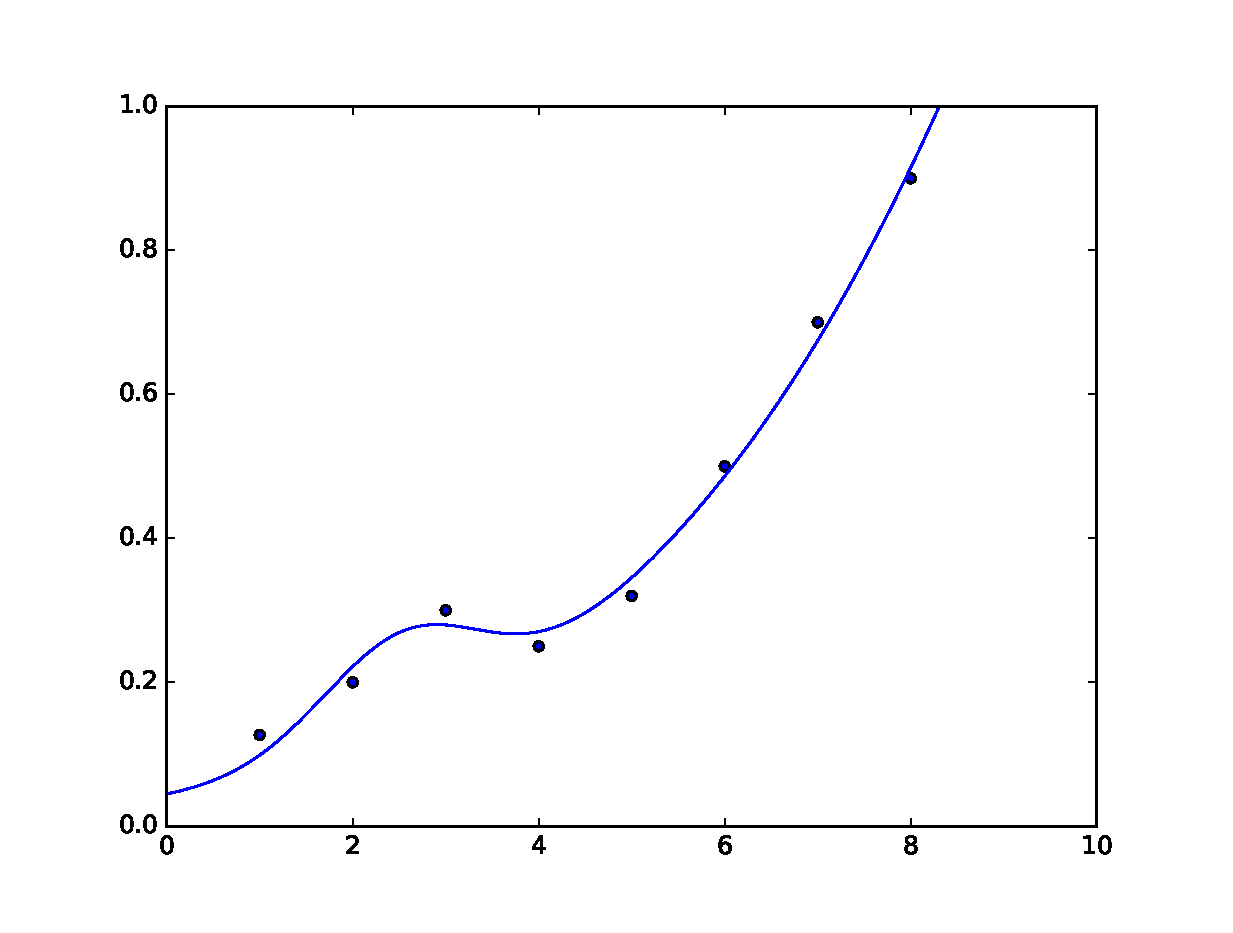
\includegraphics[scale=0.6]{levenberg-marquardt}
   \end{center}
   \caption{\label{étiquette} Points de données $\lbrace(x_i,y_i)\rbrace_i$ et la fonction d'approximation correspondante}
\end{figure}

L'algorithme converge en $31$ itérations avec $\frac{\left\|\nabla J(\textbf{u}^k)\right\|}{\left\|\nabla J(u^0)\right\|} \leq 10^{-4}$. On remarque de plus que la fonction passe près des points. 

\section{Méthode sans gradient. Algorithme de Nelder-Mead}
Le nombre d'évaluation nécessaire pour atteindre une précision de $\frac{\left\|\nabla J(\textbf{u}^k)\right\|}{\left\|\nabla J(u^0)\right\|} \leq 10^{-4e}$ est de $46$ itérations. On peut d'ailleurs remarquer que la condition d'arrêt semble absurde car elle requiert de calculer le gradient de la fonction $J$ alors que tout l'intérêt de cette méthode est de s'en passer, on pourrait utiliser le test classique $\left\| u^{k+1}-u^k\right\| \leq 10^{-4}$.

\begin{figure}[h]
 	\begin{center}
   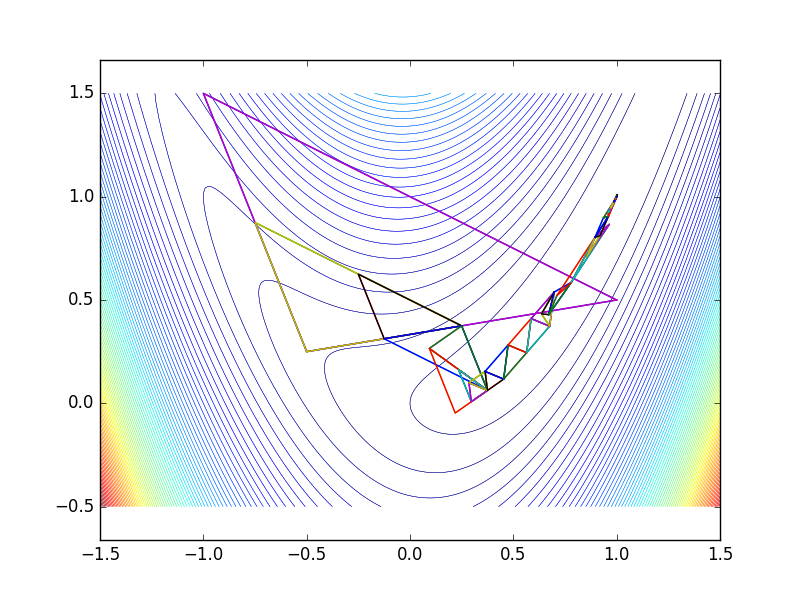
\includegraphics[scale=0.6]{nelder-mead}
   \end{center}
   \caption{\label{étiquette} Points de données $\lbrace(x_i,y_i)\rbrace_i$ et la fonction d'approximation correspondante}
\end{figure}








\end{document}e